\documentclass[12pt,a4paper]{article}
\usepackage[utf8]{inputenc}
\usepackage{graphicx}
\usepackage{geometry}
\usepackage{listings}
\usepackage{xcolor}
\usepackage{hyperref}
\geometry{a4paper, margin=1in}

\title{\textbf{Foundation Of Computer Systems Assignment 2} \\ \Large The Plaksha Orbital Pipeline Deck !!}
\author{Kanishk Khandelwal, Garvit Jain, Suyash Prakash}
\date{\today}

\begin{document}

\maketitle

\section{Introduction}
The Plaksha Orbital Pipeline Deck is a highly visual, interactive RISC Pipeline Hazard Simulator developed from first principles. It models the execution of instructions through 4-stage and 5-stage pipelines, detecting and resolving Read-After-Write (RAW) data hazards and Load-Use penalties down to the exact clock cycle.

\section{Design of the Applet}
The application is structured into two main components:
\begin{itemize}
    \item \textbf{Frontend (Cyber-IDE UI):} Built with vanilla HTML, CSS, and JavaScript, the interface features a modern developer "IDE" aesthetic. It utilizes colored, rounded "pills" to represent instructions dynamically flowing through pipeline stages in a responsive, floating timeline grid.
    \item \textbf{Backend Simulation Engine (\texttt{pipeline.js}):} A custom state machine that processes the lifecycle of instructions. Instead of hardcoding visual strings, it dynamically computes a robust \texttt{history} matrix where each instruction physically progresses through \texttt{IF $\rightarrow$ ID $\rightarrow$ EX $\rightarrow$ MEM $\rightarrow$ WB} states.
\end{itemize}

\section{Assumptions in the Simulation}
\begin{itemize}
    \item \textbf{In-Order Execution:} Instructions are fetched, decoded, and retired strictly in-order.
    \item \textbf{Single-Issue Pipeline:} Only one instruction can be fetched and processed per clock cycle.
    \item \textbf{Symbolic Execution:} The simulator models architectural timing and hazard dependencies rather than performing raw arithmetic value computation.
    \item \textbf{Simulation Bounds:} To prevent infinite loops on malformed inputs, the simulator safely caps execution at a maximum of 50 cycles or 10 active instructions.
    \item \textbf{Structural Hazards:} We assume structurally independent instruction and data memory units, preventing structural hazards during concurrent \texttt{IF} and \texttt{MEM} stages.
\end{itemize}

\section{Supported Instruction Format}
The simulator parses and supports standard MIPS/RISC-like instruction syntax via dynamic Regular Expressions:
\begin{itemize}
    \item \textbf{3-Operand Arithmetic/Logical:} \texttt{OP dest, src1, src2} (e.g., \texttt{ADD}, \texttt{SUB}, \texttt{MUL}, \texttt{AND}, \texttt{OR}, \texttt{XOR})
    \item \textbf{Immediate Arithmetic:} \texttt{OP dest, src1, imm} (e.g., \texttt{ADDI}, \texttt{ORI})
    \item \textbf{Memory Instructions:} 
    \begin{itemize}
        \item Load: \texttt{LW dest, offset(base\_reg)}
        \item Store: \texttt{SW src, offset(base\_reg)}
    \end{itemize}
\end{itemize}

\section{Hazard Detection and Resolution Logic}
Hazard detection is localized entirely within the \textbf{Decode (ID) stage gateway}. Before an instruction is permitted to transition from \texttt{ID} to \texttt{EX}, the engine invokes a \textit{backward-scanning algorithm}.

\subsection{Detection Mechanism}
The engine iterates backward through the pipeline history to find younger, un-retired instructions currently occupying the \texttt{EX}, \texttt{MEM}, or \texttt{WB} stages. It then checks if the \texttt{dest} (destination) register of any older instruction matches the required \texttt{src} (source) registers of the current instruction.

\subsection{Resolution Mechanism}
\begin{itemize}
    \item \textbf{Without Forwarding:} A \texttt{STALL} bubble is immediately issued. The dependent instruction remains locked in the \texttt{ID} stage (and pushes \texttt{STALL} visually) until the older instruction reaches the \texttt{WB} stage (or \texttt{MEM\_WB} for a 4-stage pipeline).
    \item \textbf{With Forwarding Enabled:} 
    \begin{itemize}
        \item If the older instruction is a standard ALU operation (e.g., \texttt{ADD}), the data is dynamically bypassed. The dependent instruction proceeds directly to \texttt{EX} without stalling.
        \item If the older instruction is \texttt{LW} and is currently in \texttt{EX}, a \textbf{Load-Use Penalty} occurs. A single \texttt{STALL} is inserted, allowing the \texttt{LW} instruction to finish its \texttt{MEM} stage so the loaded data can be successfully forwarded on the subsequent cycle.
    \end{itemize}
\end{itemize}

\section{Running the Applet}
\begin{enumerate}
    \item Open \texttt{index.html} in any modern web browser (no local server required).
    \item In the left-hand \textbf{Editor} pane, enter a sequence of assembly instructions.
    \item In the \textbf{Configuration} pane, select the desired pipeline model (4-Stage or 5-Stage) and toggle Data Forwarding ON or OFF.
    \item Click \textbf{Run Simulation} to instantly compute and render the timeline, or use \textbf{Step Cycle} to advance the clock manually and watch hazards resolve in real-time.
\end{enumerate}

\section{Screenshots}
\begin{figure}[h]
    \centering
    % Ensure screenshot.png is in the same directory as the .tex file
    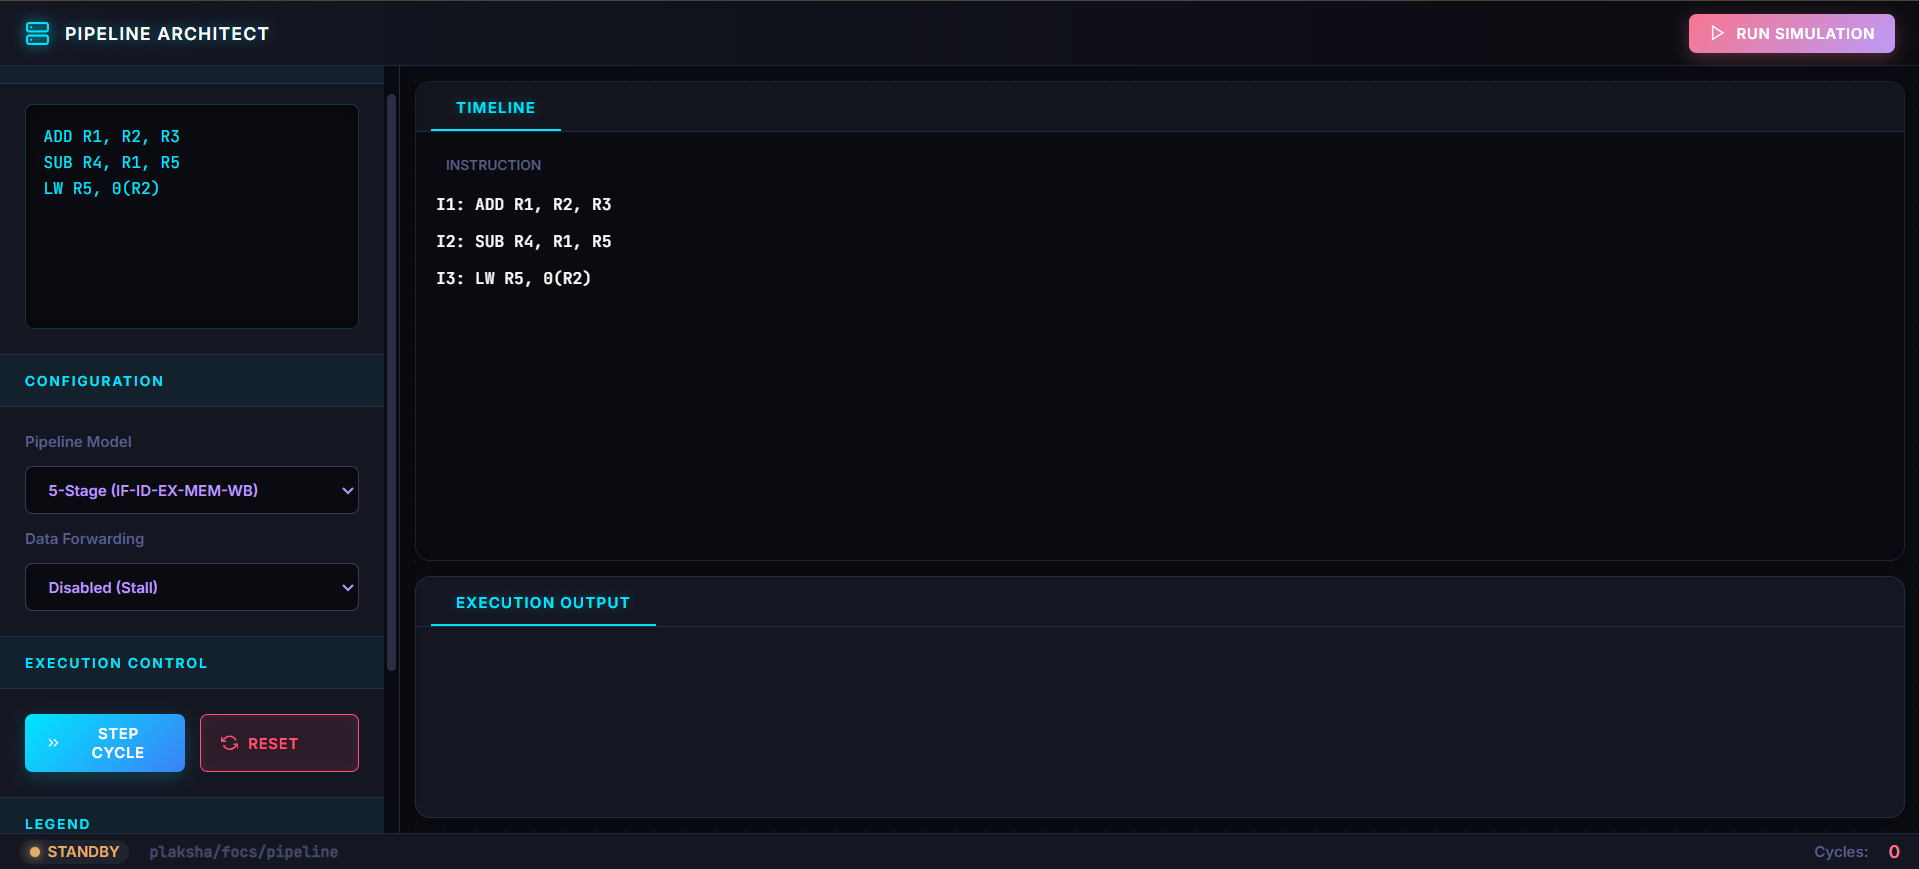
\includegraphics[width=\textwidth]{screenshot.png}
    \caption{The Pipeline Architect Interface resolving a Data Hazard.}
    \label{fig:interface}
\end{figure}

\section{Sample Test Cases}
\subsection{Test Case 1: RAW Hazard (No Forwarding)}
\textbf{Input:}
\begin{verbatim}
ADD R1, R2, R3
SUB R4, R1, R5
\end{verbatim}
\textbf{Behavior:} The \texttt{SUB} instruction stalls in \texttt{IF}/\texttt{ID} for exactly 2 cycles until the \texttt{ADD} instruction reaches its \texttt{WB} stage, ensuring \texttt{R1} is safely written back to the register file before being read.

\subsection{Test Case 2: Data Forwarding Bypass}
\textbf{Input:}
\begin{verbatim}
ADD R1, R2, R3
SUB R4, R1, R5
\end{verbatim}
\textbf{Behavior (Forwarding Enabled):} The \texttt{SUB} instruction does not stall. Instead, the \texttt{ID} stage reads the bypassed data directly from the \texttt{EX}/\texttt{MEM} pipeline registers, allowing the instruction to proceed to \texttt{EX} immediately.

\subsection{Test Case 3: Load-Use Penalty}
\textbf{Input:}
\begin{verbatim}
LW R1, 0(R2)
ADD R3, R1, R4
\end{verbatim}
\textbf{Behavior (Forwarding Enabled):} A Load-Use hazard is detected. \texttt{ADD} is stalled for exactly 1 cycle (\texttt{STALL}) because \texttt{R1} cannot be forwarded until \texttt{LW} finishes fetching data from memory in its \texttt{MEM} stage. Data is then forwarded perfectly on the subsequent cycle.

\end{document}
